\subsection{Elliptic Problems}

For elliptic problems, the speed of the propagation is infinite and thus responds instantly to any change the source or boundary conditions. For these sorts of problems, relaxation methods work well, but techniques like multigrid can speed things up. 

Lets consider a problem that arises in astrophysics and electrostatics, the Poisson equation
\be
\nabla^2\Phi = f
\ee
Let's consider the 1-d version first 
\be
\dddx\Phi = f
\ee
with boundary conditions $\Phi(0) = \Phi(1) = 0$.  If we pick $f=\sin(x)$, then we have an analytic solution $\Phi = -\sin(x) +x\sin(1)$.  Given this, how can we solve for this numerically.  

Fortunately, this is an ODE and so the first technique that we will try is using one of our ODE integrators -- say rk2.  Now if we use rk2, we start our and $x=0$ and integrate to $x=1$.  Since $\Phi(x=0) = 0$, we have one initial condition already, but we will need another initial condition for $\Phi'(x=0)$.  We can set this to be a free value, say $\alpha$ and vary it until we get the second boundary condition.  

In other works, lets define a function $g(\alpha)$ such that
\be
g(\alpha) = \Phi(x=1;\alpha),
\ee
where $\Phi$ is computed by numerical integration to $x=1$ using $\Phi'(x=0) = \alpha$.  Since we want $g(\alpha) = 0$, this reduces to a root-finding problem for $\alpha$.  So once we define $g(\alpha)$, we can use root finding routines to find the appropriate value of $\alpha$.  For this, we will use a standard python package. This technique is known as shooting as you are essential shooting until you hit a target.  

\lstinputlisting[language=Python]{code/shoot.py}

Shooting doesn't always work especially with stiff equations which are extremely sensitive to initial conditions.  Examples of this in astrophysics include hydrostatic balance for stars.  In this case, we need to try something different.  Lets discretize the equation to be
\be
\frac{\Phi_{i+1} - 2\Phi_i + \Phi_{i-1}}{\Delta x^2} = f_i,
\ee
where we pick $\Phi_0 = \Phi_N = 0$.  We then have a bunch of algebraic equations:
\be
\Phi_i = 0.5\left(\Phi_{i+1} + \Phi_{i-1} - \Delta x^2 f_i\right).
\ee
In principle, we can solve with matrix inversion, but it is easier to solve using relaxation starting with some initial guess $\Phi_i^0$  This can use either 
\begin{enumerate}
    \item Jacobi iteration: $\Phi_i^{k+1} = 0.5\left(\Phi_{i+1}^k + \Phi_{i-1}^k - \Delta x^2 f_i\right).$
    \item Gauss-Seidel iteration: Use the new $k+1$ values as they appear. 
\end{enumerate}
In either case, you need to keep track of the error to ensure that the error goes down below some threshold. 

Lets look at the code here.
\lstinputlisting[language=Python]{code/relax.py}

which yields the following compared to the analytic result:
\begin{figure}
    \centering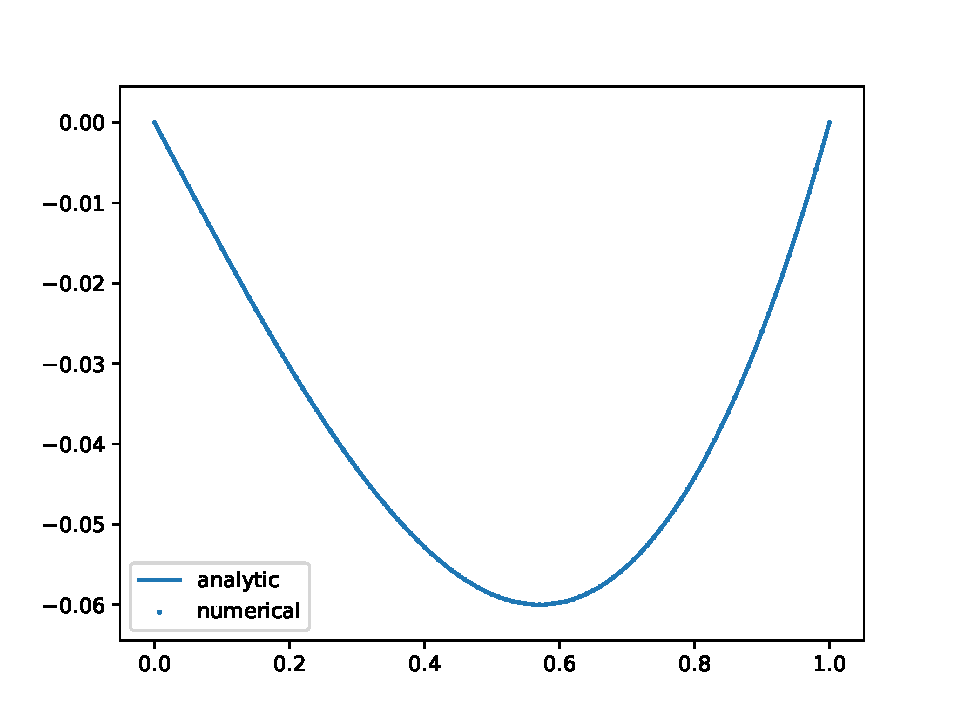
\includegraphics[width=0.75\textwidth]{code/relax.pdf}
    \caption{\label{fig:relax}}
\end{figure}

Running this you can see that theres are quite a few iteration needs to solve this equation. This can be accelerated by coarsening and then refining the grid in a technique known as multigrid. We won't cover this in this as in astrophysics there are other ways to solve this equation (FFTs for instance).